\documentclass[11pt, aspectratio=169]{beamer}
% \documentclass[11pt,handout]{beamer}
\usepackage[T1]{fontenc}
\usepackage[utf8]{inputenc}
\usepackage{textcomp}
\usepackage{float, afterpage, rotating, graphicx}
\usepackage{epstopdf}
\usepackage{longtable, booktabs, tabularx}
\usepackage{fancyvrb, moreverb, relsize}
\usepackage{eurosym, calc}
\usepackage{amsmath, amssymb, amsfonts, amsthm, bm}
\usepackage[
    natbib=true,
    bibencoding=inputenc,
    bibstyle=authoryear-ibid,
    citestyle=authoryear-comp,
    maxcitenames=3,
    maxbibnames=10,
    useprefix=false,
    sortcites=true,
    backend=biber
]{biblatex}
\AtBeginDocument{\toggletrue{blx@useprefix}}
\AtBeginBibliography{\togglefalse{blx@useprefix}}
\setlength{\bibitemsep}{1.5ex}
\addbibresource{../refs.bib}

\hypersetup{colorlinks=true, linkcolor=black, anchorcolor=black, citecolor=black,
filecolor=black, menucolor=black, runcolor=black, urlcolor=black}

\setbeamertemplate{footline}[frame number]
\setbeamertemplate{navigation symbols}{}
\setbeamertemplate{frametitle}{\centering\vspace{1ex}\insertframetitle\par}

\newcommand{\indep}{\perp\!\!\!\!\perp}

\AtBeginSection[]{
  \begin{frame}
  \vfill
  \centering
  \begin{beamercolorbox}[sep=8pt,center,shadow=true,rounded=true]{title}
    \usebeamerfont{title}\insertsectionhead\par%
  \end{beamercolorbox}
  \vfill
  \end{frame}
}

\newcommand{\backupbegin}{
   \newcounter{framenumberappendix}
   \setcounter{framenumberappendix}{\value{framenumber}}
}
\newcommand{\backupend}{
   \addtocounter{framenumberappendix}{-\value{framenumber}}
   \addtocounter{framenumber}{\value{framenumberappendix}}
}

\title{Inference in Partially Identified Marginal Treatment Effect Models}
\subtitle{BGSE Brown Bag Presentation}
\author[Julian Budde]{\bf Julian Budde}

\begin{document}



\begin{frame}
    \titlepage
    \note{~}
\end{frame}

\begin{frame}
    \frametitle{Motivation}

    \citet{mogstad2018using} propose partial identification approach for \textit{extrapolating} information from instrumental variable estimates

    \vspace{0.5cm}

    Focus is on identification and estimation

    \vspace{0.5cm}

    Less on \textit{inference}:

    \vspace{0.5cm}
    \pause
    \begin{itemize}
        \footnotesize
        \item Working paper version has an inference procedure \dots
        \item \dots but no simulation results and no implementation.
        \pause
        \item Authors' \textit{R package} supports bootstrap and subsampling \dots
        \item \dots but ``[t]here does not currently exist a solution for the MTE framework that is both theoretically
        satisfactory and computationally tractable\dots [implemented methods] are known to not be valid in general''
    \end{itemize}

    \vspace{0.5cm}
    No simulation results.

\end{frame}

\begin{frame}
    \begin{figure}
        
\includegraphics[height=0.75\textheight]{mt_handbook_table6.png}
        \caption{\citet{mogstad2024instrumental} Handbook Chapter}
    \end{figure}
\end{frame}

\begin{frame}
    \frametitle{This Project}

        Show the standard bootstrap is invalid in simple MTE model.
        \begin{itemize}
            \item Look at some alternative approaches.
        \end{itemize}

        \vspace{0.5cm}

        Simulation results for coverage probabilities in empirically relevant setting.

        \vspace{0.5cm}

        Suggest approach for conservative inference using relaxed optimization problem.

\end{frame}

\begin{frame}
    \tableofcontents
\end{frame}

\section{Background: MTE Approach}

\begin{frame}
    \frametitle{MTE Approach}

    Program evaluation setting:
    \begin{itemize}
        \item Outcome $Y$
        \item Binary Treatment $D$ and Instrument $Z$
    \end{itemize}

    \vspace{0.5cm}

    Want to construct identified set for a target parameter.

    \vspace{0.5cm}
    We use
    \begin{itemize}
        \item Information in the data: Point-identified estimands.
        \item Economic reasoning: Shape restrictions and parametric assumptions.
    \end{itemize}

\end{frame}

\begin{frame}
    \frametitle{MTE Approach: Latent Heterogeneity}

    \textbf{Treatment Choice Equation}:
    \begin{equation*}
        D = I\{p(Z) - U \geq 0\}
    \end{equation*}
    $U\indep Z$, $U\sim Unif[0,1]$.

    \vspace{0.5cm}

    $U$ is ``resistance'' to treatment: Small $u$ $\rightarrow$ always take treatment.

    \vspace{0.5cm}

    Three groups: \textit{always-taker} $[0, p(1)]$, \textit{complier} $[p(0), p(1)]$, \textit{never-taker} $[p(0), 1]$.

    \vspace{0.5cm}
    \pause
    Key to the paper: Define everything in terms of unobservable MTR functions.

    \begin{equation*}
        m_d(u) \equiv E[Y_d | U=u] \quad \text{ for } d\in\{0, 1\}.
    \end{equation*}

\end{frame}

% \begin{frame}
%     \frametitle{MTE Model: Assumptions}
%     $(Y,D,Z)$ are observable, $(Y_1, Y_0, U)$ unobservables.


%     \begin{itemize}
%         \item $U \indep Z$
%         \item $E[Y_d|Z,U] = E[Y_d|U]$ and $E[Y_d^2] < \infty$ for $d \in \{0,1\}$
%         \item $U$ is uniform on $[0,1]$ conditional on $Z$.
%     \end{itemize}

% \end{frame}

\begin{frame}
    \frametitle{MTE Approach: Linear Program}

    Find the largest target parameter


    \begin{equation*}
        \overline{\beta^*} = \underbrace{\sup_{(\theta_0, \theta_1) \in \Theta}}_{\substack{\text{Maximize over} \\ \text{bfunc coefs.}}}\sum_{k=1}^{K_0} \theta_{0k}\overbrace{\Gamma^*_0(b_{0k})}^{\substack{\text{Map from} \\ \text{MTR to } \beta^*.}} + \sum_{k=1}^{K_1} \theta_{1k}\overbrace{\Gamma^*_1(b_{1k})}^{\substack{\text{Map from} \\ \text{MTR to } \beta^*.}}
    \end{equation*}

    \pause

    given that

    \begin{equation*}
        \sum_{k=1}^{K_0} \theta_{0k}\Gamma_{0s}(b_{0k}) + \sum_{k=1}^{K_1} \theta_{1k} \Gamma_{1s}(b_{1k}) = \beta_s \quad \text{ for all } s\in\mathcal{S}.
    \end{equation*}

    \vspace{0.5cm}
    $\beta_s$ and all $\Gamma$ are point-identified.
    $\Theta$ incorporates all shape restrictions.

\end{frame}

\begin{frame}
    \frametitle{MTE Approach: Example}

    \only<1>{
        Find the largest target parameter


        \begin{equation*}
            \overline{\beta^*} = \sup_{(\theta_0, \theta_1) \in \Theta}\sum_{k=1}^{K_0} \theta_{0k}\Gamma^*_0(b_{0k}) + \sum_{k=1}^{K_1} \theta_{1k}\Gamma^*_1(b_{1k})
        \end{equation*}
        }
    \only<2,3,4,5>{
        Find the largest \textcolor{red}{ATE}

    \begin{equation*}
        \overline{\beta^*} = \sup_{(\theta_0, \theta_1) \in \Theta}
        \sum_{k=1}^{K_0} \theta_{0k}\textcolor{red}{(-1) \int_0^1 b_{0k}(u)du}
        + \sum_{k=1}^{K_1} \theta_{1k} \textcolor{red}{(1) \int_0^1 b_{1k}(u)du}
    \end{equation*}
    }

    given \only<1,2>{that}\only<3,4,5>{the \textcolor{red}{IV slope}}
    \only<1,2>{
        \begin{align*}
            &\sum_{k=1}^{K_0} \theta_{0k}\Gamma_{0s}(b_{0k}) \\
            &+ \sum_{k=1}^{K_1} \theta_{1k} \Gamma_{1s}(b_{1k}) = \beta_s \quad \text{ for all } s\in\mathcal{S}.
        \end{align*}
        }

        \only<3>{
            \begin{align*}
                &\sum_{k=1}^{K_0} \theta_{0k}\Gamma_{0s}(b_{0k}) \\
                &+ \sum_{k=1}^{K_1} \theta_{1k} \Gamma_{1s}(b_{1k}) = \textcolor{red}{\frac{Cov(Y,D)}{Var(D)}}
    \end{align*}
    }

        \only<4,5>{
            \begin{align*}
            &\sum_{k=1}^{K_0} \theta_{0k}\textcolor{red}{E\left[\int_0^1 b_{0k}(u)\frac{Z - E[Z]}{Cov(D,Z)}I\{u > p(Z)\}du\right]} \\
            &+ \sum_{k=1}^{K_1} \theta_{1k} \textcolor{red}{E\left[\int_0^1 b_{1k}(u)\frac{Z - E[Z]}{Cov(D,Z)}I\{u\leq p(Z)\}du\right]} = \textcolor{red}{\frac{Cov(Y,D)}{Var(D)}}
    \end{align*}
    }

    \vspace{0.5cm}

    \only<1,2,3,4>{
    $\Theta$ incorporates all shape restrictions.
    }

    \only<5>{
    \textcolor{red}{Outcome bounds}: $Y\in[0,1] \Rightarrow \Theta = [0,1]^{K_0 + K_1}$.
    }

\end{frame}

\section{Bootstrap Invalidity: Simple Example}

\begin{frame}
    \frametitle{Setup}

    \begin{itemize}
        \item Outcome $Y \in [0,1]$, $D$ and $Z$ binary
        \item $0 \leq p_0 < p_1 \leq 1$.
    \end{itemize}

    \vspace{0.5cm}

    \textbf{Point-Identified}: $\beta_s = E[Y_1 - Y_0 | u \in (p_0, p_1]]$.

    \vspace{0.5cm}

    \textbf{Target Parameter}: $\beta^* = E[Y_1 - Y_0 | u \in (p_0, p_1 + \overline{u}]]$.

    \vspace{0.5cm}

    No parametric assumptions on basis functions.

\end{frame}

\begin{frame}
    \frametitle{Solution}

    Let $\beta_{\overline{u}} \equiv E[Y(1) - Y(0) | u \in [p_1, p_1 + \overline{u}]]$.

    \vspace{0.5cm}

    Then $\beta^*$ is a weighted average of the two LATEs:\@

    \begin{equation*}
        \beta^* = \omega\beta_s + (1-\omega)\beta_{\overline{u}}
    \end{equation*}

    where $\omega = \frac{p_1 - p_0}{\overline{u} + p_1 - p_0}$ is the relative complier share.

    \vspace{0.5cm}

    $\Rightarrow$ Find bounds on $\beta_{\overline{u}}$.

\end{frame}

\begin{frame}
    \frametitle{Solutions}

    \textbf{Bounded Outcome}:
    \begin{equation*}
        \beta^* \in [\omega\beta_s - (1 - \omega), \omega\beta_s + (1 - \omega)]
    \end{equation*}

    \vspace{0.5cm}

    \pause

    \textbf{Decreasing Marginal Treatment Effect}:
    \begin{equation*}
        \beta^* \in [\omega\beta_s - (1 - \omega), \beta_s]
    \end{equation*}

    \vspace{0.5cm}
    \pause

    % \textbf{Positive Treatment Response}:
    % \begin{equation*}
    %     \beta^* \in \begin{cases}
    %         [\omega\beta_s, \beta_s + (1 - \omega)] & \beta_s \geq 0 \\
    %         \emptyset & \beta_s < 0
    %     \end{cases}
    % \end{equation*}

% \end{frame}

% \begin{frame}
%     \frametitle{Solutions: Constant Splines II}

    \textbf{Decreasing Marginal Treatment Response}:

    % \begin{equation}\label{eq:solution_cs_increasing_mtr_upper}
    %     \overline{\beta^*}(\beta_s, \omega)=
    %     \begin{cases}
    %         \omega \beta_s + (1 - \omega),& \quad \text{if } \beta_s \geq 0\\
    %         \beta_s + (1 - \omega),              & \quad \text{if } \beta_s < 0,
    %     \end{cases}
    % \end{equation}
    % and
    \begin{equation}\label{eq:solution_cs_increasing_mtr_lower}
        \underline{\beta^*}(\beta_s, \omega)=
        \begin{cases}
            \beta_s - (1 - \omega),& \quad \text{if } \beta_s \geq 0\\
            \omega \beta_s - (1 - \omega),              & \quad \text{if } \beta_s < 0.
        \end{cases}
    \end{equation}

\end{frame}

\begin{frame}
    \begin{figure}
        \includegraphics[height=0.85\textheight]{../../bld/figures/binary_iv/id_constant_nan_shape_constraints_late_['lower', 'upper'].png}
    \end{figure}
\end{frame}

\begin{frame}[label=infsimple]
    \frametitle{Inference}

    The \textit{standard bootstrap} fails at the kinks (e.g.~\citet{fang2019infdirdiff}).

    \vspace{0.5cm}

    \textbf{Alternatives}: Based on \textit{directional} differentiability of $\phi$ we can use adjusted delta methods.
    \begin{itemize}
        \item \textit{Analytical} delta method, e.g.~\cite{fang2019infdirdiff}.
        \item \textit{Numerical} delta method, e.g.~\cite{hong2018numerical}.
    \end{itemize}

    \vspace{0.5cm}
    Use the following approximation:
    \begin{equation*}
        \sqrt{N}\left({\overline{\beta^*}(\hat{\beta}_s)} - \overline{\beta^*}(\beta_s)\right) \approx \overline{\beta^*}'\left(\sqrt{N}\left(\hat{\beta}_n - \beta_0\right)\right)
    \end{equation*}

    \footnotesize  \hyperlink{analytical_delta}{\beamerbutton{Details}}

\end{frame}

\begin{frame}
    \frametitle{Monte Carlo Simulations}

    \begin{itemize}
        \item True parameter $\beta^*$ at upper bound of identified set.
        \item Compare: Standard bootstrap, analytical and numerical delta method.
    \end{itemize}

    \vspace{0.5cm}

    To construct $1-\alpha = 0.95$ confidence interval for \textit{true parameter}:
    \begin{itemize}
        \item Quantiles from (adjusted) bootstrap.
        \item One-sided $\alpha$ intervals for upper and lower bound \citep{imbens2004confidence}.
    \end{itemize}

    \vspace{0.5cm}

    DGP\@: $p_0 = 0.4 < 0.6 = p_1$, $P(Z=0)=0.5$, $Y(d) = \gamma_d^g + \epsilon$ with $\epsilon\sim N(0, \sqrt{0.1})$.

    % \vspace{0.5cm}
    % $s_n = 1 / \sqrt{n}$, $\kappa_n = \sqrt{\ln(n)}$.

\end{frame}

\begin{frame}
    \frametitle{Simple Monte Carlo: Coverage}

    \begin{figure}
        \includegraphics[height=0.75\textheight]{../../bld/simple_model/figures/coverage.png}
    \end{figure}

\end{frame}

\begin{frame}
    \frametitle{Simple Monte Carlo: Length}

    \begin{figure}
        \includegraphics[height=0.75\textheight]{../../bld/simple_model/figures/length.png}
    \end{figure}

\end{frame}

\section{Simulation Studies: More Realistic Example}

\begin{frame}
    \frametitle{Simulation Studies}
    Goal: Simulation study closer to empirical application.

    \vspace{0.5cm}

    \begin{itemize}
        \item Sharp identified set.
        \item Flexible polynomial for MTR functions.
        \item Shape restrictions.
    \end{itemize}

    \pause

    \vspace{0.5cm}

    (Minor) difficulty: Construct DGP \textit{consistent} with assumptions and with \textit{parameter at boundary} of ID set.

    \vspace{0.5cm}

    For now just \textit{nonparametric bootstrap} and \textit{subsampling}.

\end{frame}

\begin{frame}{Solutions: Bernstein Polynomials ($k=2$)}

    \begin{figure}
        \centering
        \includegraphics[height=0.825\textheight]{../../bld/figures/binary_iv/id_bernstein_2_mte_monotone_sharp_lower.png}
    \end{figure}


\end{frame}

\begin{frame}{Solutions: Bernstein Polynomials ($k=11$)}

    \begin{figure}
        \centering
        \includegraphics[height=0.825\textheight]{../../bld/figures/binary_iv/id_bernstein_11_mte_monotone_sharp_lower.png}
    \end{figure}


\end{frame}


% \begin{frame}
%     \frametitle{DGP\@: Construction}

%     \textbf{Parameters}: $\gamma_d^g = E[Y_d|g(U)=g]$ with $d\in\{0,1\}$ and $g = \{at, c, nt\}$.

%     \vspace{0.5cm}

%     \footnotesize{Cannot just take $\gamma_1^{nt} - \gamma_0^{nt} = -1$.}

%     \vspace{0.5cm}

%     \normalsize

%     \textbf{Step 1}: Fix point-identified $\gamma_1^{at}, \gamma_1^c, \gamma_0^c, \gamma_0^{nt}$. Solve population problem with Bernstein basis functions and all constraints.

%     \vspace{0.5cm}

%     \textbf{Step 2}: Use the population solutions $m_d(u;\gamma)$ for the lower bound to construct a DGP\@.

%     \vspace{0.5cm}

%     \footnotesize{Polynomials that imply $\gamma_1^{nt}, \gamma_0^{nt}$.}

%     \vspace{0.5cm}
%     \normalsize

%     Simulation: $Y_i = D_i m_1(u;\gamma) + (1-D_i)m_0(u;\gamma) + \epsilon_i$.

% \end{frame}

\begin{frame}
    \frametitle{DGP}

    \textbf{Parameters}: $\gamma_d^g = E[Y_d|g(U)=g]$ with $d\in\{0,1\}$ and $g = \{at, c, nt\}$.

    \vspace{0.5cm}

    View as function of LATE\@: $\gamma_1^c = \beta_s/2 + 0.5$, $\gamma_0^c = -\beta_s/2 + 0.5$.

    \vspace{0.5cm}

    Set $\gamma_1^{at} = 0.75$ and $\gamma_0^{nt} = 0.2$.

    \vspace{0.5cm}

    Simulation: $Y_i = D_i m_1(u;\gamma) + (1-D_i)m_0(u;\gamma) + \epsilon_i$.

    \only<2>{

    \vspace{0.5cm}

    Results for the \textit{non-parametric bootstrap} and \textit{subsampling} ($B = 0.1\times N$).\footnote{
        Use own Python implementation hosted at {\href{https://github.com/buddejul/pyvmte}{github.com/buddejul/pyvmte}}.
    }
    }

\end{frame}

\begin{frame}
    % \frametitle{Result: Consistency}

    \begin{figure}
        \includegraphics[height=0.95\textheight]{../../bld/figures/pyvmte_sims/1n/sims_binary_iv_sharp_mte_monotone_means_bootstrap.png}
    \end{figure}

\end{frame}

\begin{frame}

    \begin{figure}
        \includegraphics[height=0.95\textheight]{../../bld/figures/pyvmte_sims/1n/sims_binary_iv_sharp_mte_monotone_coverage.png}
    \end{figure}

\end{frame}

\begin{frame}
    \frametitle{Simulation Results: Variations}
    Undercoverage is also observed for
    \begin{itemize}
        \item all other shape constraints;
        \item different subsample size ($s\in\{0.05, 0.1, 0.2\}$);
        \item critical values adjusted for the length of the identified set;
        \item different linear program tolerances $(\kappa_n \in \{\frac{1}{n^2}, \frac{1}{n}, \frac{1}{\sqrt{n}}\})$.\footnote{
            Not quite true.
        }
    \end{itemize}

\end{frame}

\begin{frame}
    \frametitle{Summary}

    \textbf{Summary}: In relevant applications, confidence intervals might be severely undercovering.

    \vspace{0.5cm}

    \textbf{Caveats}: Estimator implementation, DGP\@.

    \vspace{0.5cm}

    \pause

    \textbf{Idea in thesis}: Convex relaxation. Optimize over $||x-k||_p\leq k'$ instead of $[0,1]^d$ \dots

    \vspace{0.5cm}

    \footnotesize  \hyperlink{convex_relax}{\beamerbutton{Details}}

\end{frame}

\begin{frame}[label=outlook_relax]
    \frametitle{Outlook: Inference on LP Values}

    \dots similar approaches exist:
    \begin{itemize}
        \item\citet{cho2024simple} propose \textit{perturbation} approach.

            \[\min_{x\in[0\pm\nu_1,1\pm\nu_2]^2} (c_1 \pm \epsilon_1)x_1 + (c_2 \pm \epsilon_2)x_2\]

        \item\citet{gafarov2024simple} proposes \textit{regularization} approach.

            \[\min_{x\in[0,1]^2} c_1x_1 + c_2x_2 + \mu_n||x||^2\]

        \end{itemize}
    \pause
    $\rightarrow$ Crux: \textbf{Tuning parameter choice}; maybe computational complexity.

    \vspace{0.5cm}

    Others:
    \begin{itemize}
        \item Bootstrap + pretest (\citet{bhattacharya2009inferring}, \citet{freyberger2015identification})
        \item Projection approaches
    \end{itemize}

\end{frame}

\begin{frame}

    \frametitle{Outlook: Project Direction}

    Get other approaches to work.

    \vspace{0.5cm}

    Unless MTE problem has further special structure, theory seems difficult.

    \vspace{0.5cm}

    Systematic simulation study with data from literature.

    \vspace{0.5cm}

    Extensions: Truly sharp sets \citep{marx2024sharp}, multiple instruments \citep{mogstad2024policy}.

\end{frame}


\appendix
\backupbegin

\begin{frame}[label=analytical_delta]
    \frametitle{Analytical Delta Method}

    \begin{itemize}
        \item[1.] Bootstrap approximation to distribution of $\sqrt{n}(\hat{\beta_s} - \beta_s)$.
        \item[2.] Suitable estimator $\hat{\phi'_n}$ for directional derivative.
        \item[3.] Delta method:
        \begin{equation*}
            \hat{\phi'_n}(\sqrt{n}(\hat{\beta_s}^*_n - \hat{\beta_s}_n))
        \end{equation*}
    \end{itemize}

    \vspace{0.5cm}

    In our case: Simple pre-test
    \begin{equation*}
        \hat{\phi'_n}(h)=
        \begin{cases}
            \omega h ,& \quad \text{if } \sqrt{n}\hat{\beta_s}/\hat{\sigma^s} > \kappa_n\\
            \max\{\omega h, -h\},& \quad \text{if } |\sqrt{n}\hat{\beta_s}/\hat{\sigma^s}| \leq \kappa_n\\
            h,& \quad \text{if } \sqrt{n}\hat{\beta_s}/\hat{\sigma^s} < -\kappa_n\\
        \end{cases}
    \end{equation*}
    where we require $\kappa_n \to \infty$ but more slowly than $\sqrt{n}$, i.e. $\kappa_n / \sqrt{n} \to 0$.

    \vspace{0.5cm}
    \footnotesize  \hyperlink{infsimple}{\beamerbutton{Back}}

\end{frame}

\begin{frame}
    \frametitle{Numerical Delta Method}

    Alternative: numerical approximation.
    \begin{equation*}
        \hat{\phi'}_{n, s_n} \equiv \frac{1}{s_n}\{\phi(\hat{\beta_s} + s_n h) - \phi(\hat{\beta_s})\}
    \end{equation*}

    Combining this with a bootstrap approximation to $\sqrt{n}(\hat{\beta_s} - \beta_s)$ we get
    \begin{equation*}
        \hat{\phi'}_{n, s_n}(\sqrt{n}(\hat{\beta_s} - \beta_s)) \equiv \frac{1}{s_n}\{\phi(\hat{\beta_s} + s_n \sqrt{n}(\hat{\beta_s} - \beta_s)) - \phi(\hat{\beta_s})\},
    \end{equation*}
    the distribution of which we can use to construct confidence intervals.
    We require $s_n\to0$ but $s_n\sqrt{n} \to \infty$.

    \vspace{0.5cm}
    \footnotesize  \hyperlink{infsimple}{\beamerbutton{Back}}

\end{frame}

\begin{frame}[label=convex_relax]
    \frametitle{Convex Relaxation}

    (One) problem with value of linear program is non-uniqueness of solutions.

    \begin{equation*}
        \min_{x_1, x_2\in[0,1]^d} c_1 x_1 + c_2 x_2.
    \end{equation*}

    \vspace{0.5cm}
    Assume $c_2 > 0$ known. Then the optimal value is $\phi(c_1) = \min\{0, c_1\}$.

    \vspace{0.5cm}
    Idea: Get lower bound by instead solving \textit{relaxed problem}

    \begin{equation*}
        \min_{||x-k||_p\leq k'} c_1x_1 + c_2x_2
    \end{equation*}

    Let $p\to\infty$ at appropriate rate.\\
    Might get established delta method theory for mathematical programs \citep{shapiro1991asymptotic}.
    Key question: How to choose $p$ in finite sample.

    \footnotesize  \hyperlink{outlook_relax}{\beamerbutton{Back}}

\end{frame}

\begin{frame}
    \begin{figure}
        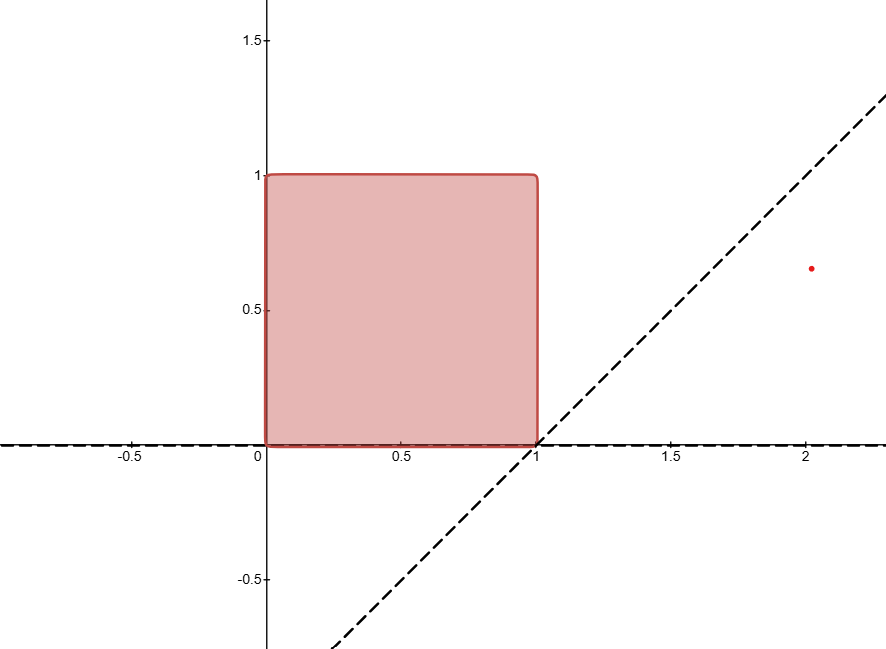
\includegraphics[height=0.9\textheight]{desmos_only_box.png}
    \end{figure}
\end{frame}

\begin{frame}
    \begin{figure}
        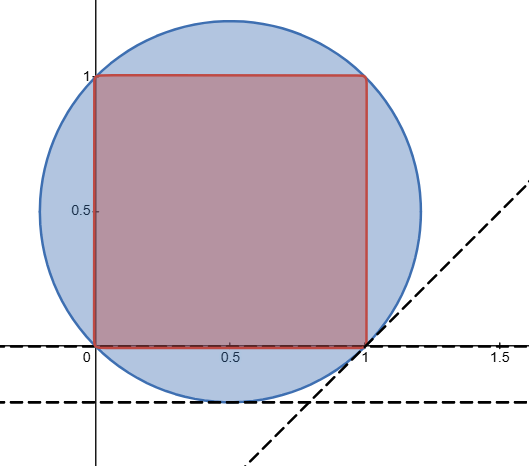
\includegraphics[height=0.9\textheight]{desmos_all.png}
    \end{figure}
\end{frame}

\begin{frame}
    \begin{figure}
        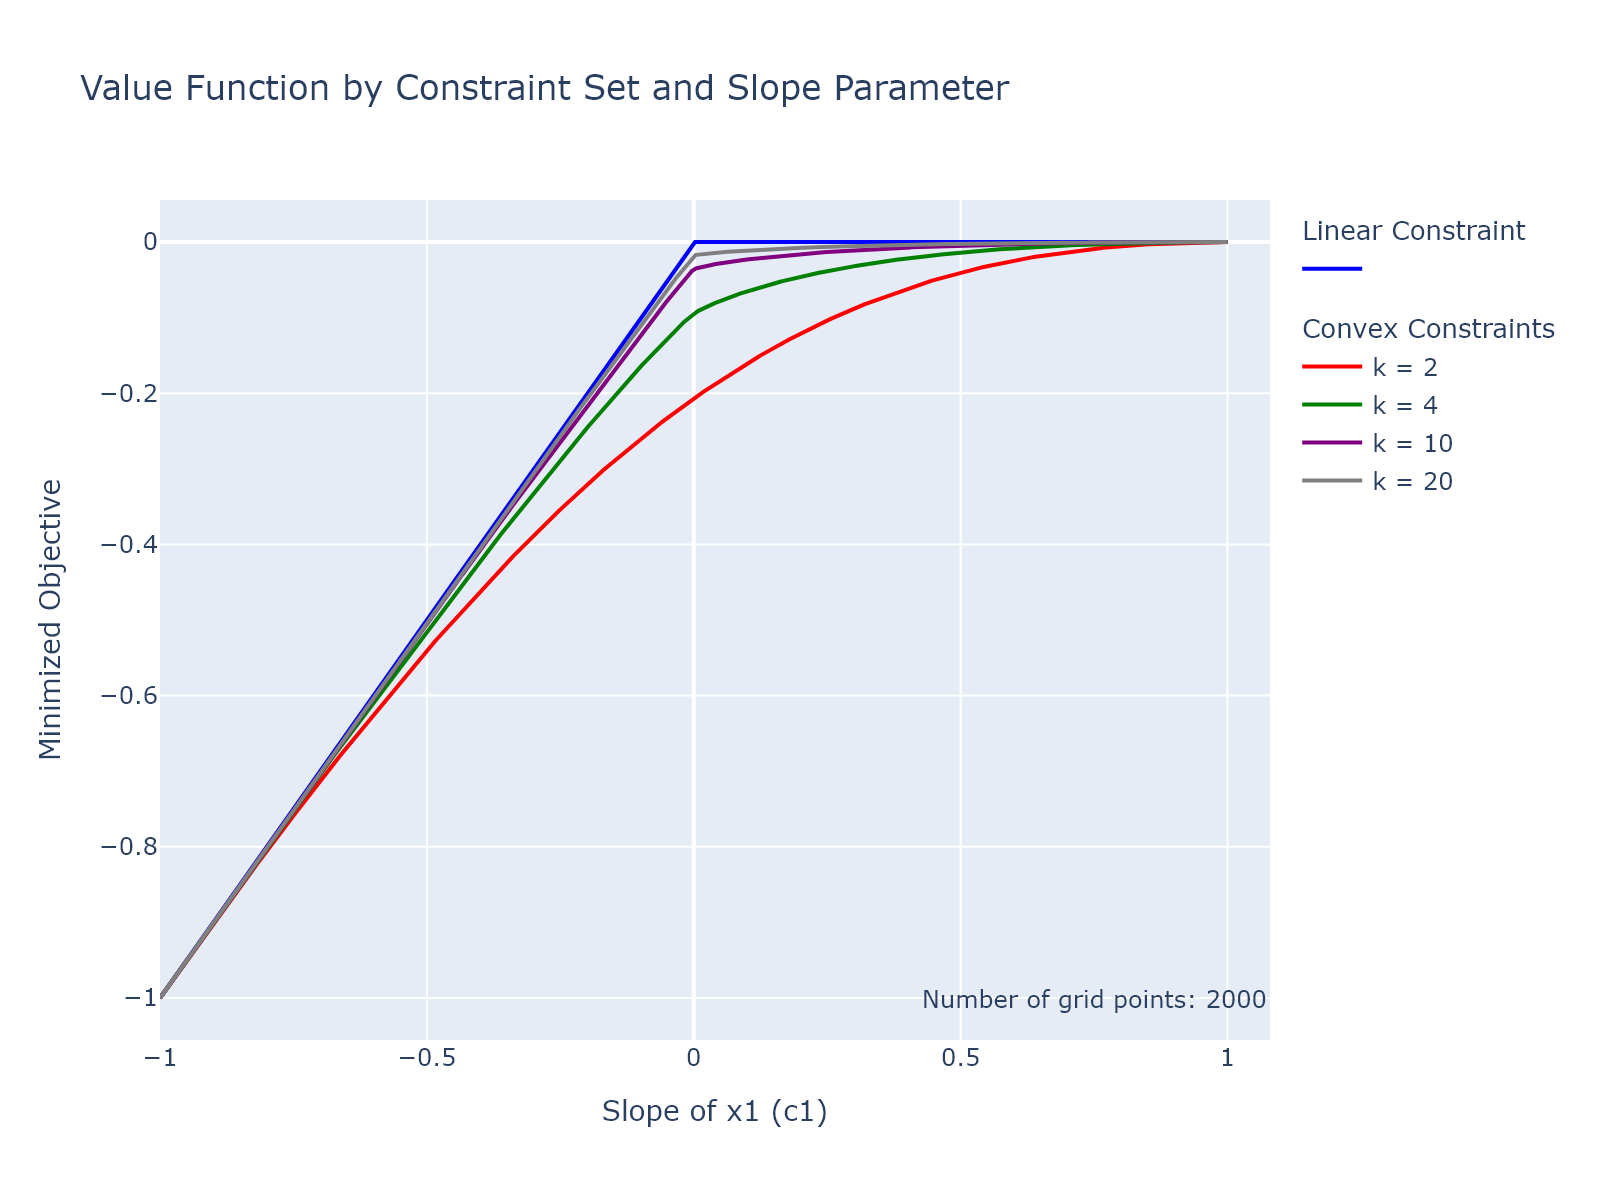
\includegraphics[height=0.9\textheight]{../figures/relax/value_function_by_constraint_set_dim_2.png}
    \end{figure}
\end{frame}

\begin{frame}
    \begin{figure}
        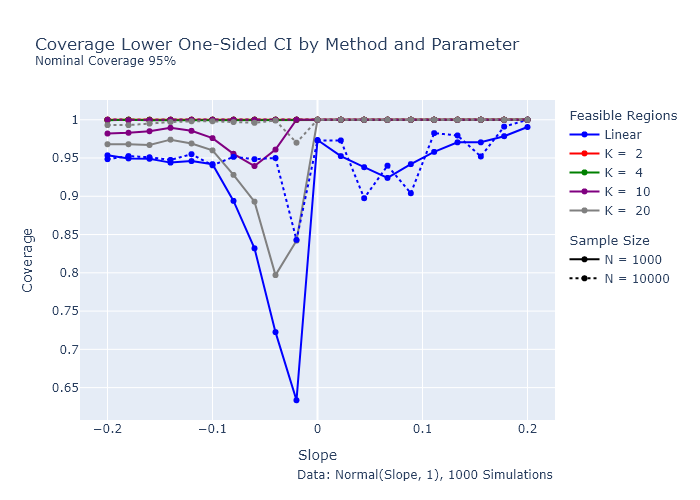
\includegraphics[height=0.9\textheight]{../figures/relax/covers_lower_one_sided_by_method.png}
    \end{figure}
\end{frame}


\begin{frame}[allowframebreaks]
    \frametitle{References}
    \renewcommand{\bibfont}{\normalfont\footnotesize}
    \printbibliography
\end{frame}

\backupend

\end{document}
